\chapter{Kategorisierung der verschiedenen Ansätze zur Entwicklung einer Mobile App}

Es existieren viele verschiedenste Kategorisierungsansätze zur Entwicklung einer mobilen App. Im Folgenden wird die Kategorisierung nach Majchrzak verwendet\cite{Majchrzak_category}. Dieser unterteilt die Entwicklung in drei unterschiedliche Ansätze, wobei auch Mischformen wie React Native, NativeScript und Flutter existieren, bei denen der Übergang zwischen den folgenden Kategorien fließend ist\cite{rieger_evaluation}. Dabei wird ein Augenmerk auf die Nutzung nativer Elemente der Zielplattform gelegt, welche auf der horizontalen Achse der \foreignlanguage{ngerman}{\cref{fig:kategorisierung_app_dev}} gekennzeichnet wurden.

\begin{enumerate}
	\item Native, plattformspezifische Entwicklung.
	\item Anwendungen welche in einer Laufzeitumgebung ausgeführt werden. Diese werden wiederum in (Progressive) Web-Apps, Hybrid-Apps und Apps, welche in ihrer eigenen Laufzeitumgebung ausgeführt werden, unterteilt.
	\item Generierende Ansätze, welche entweder auf dem Ansatz der modellgetriebenen Softwareentwicklung (Model Driven Software Development) oder dem des Cross- bzw. Transpilings basieren. Das Resultat ist dabei in jedem Fall eine native App, welche auf das \ac{SDK} des Herstellers aufbaut.
\end{enumerate}

\begin{figure}[h]
	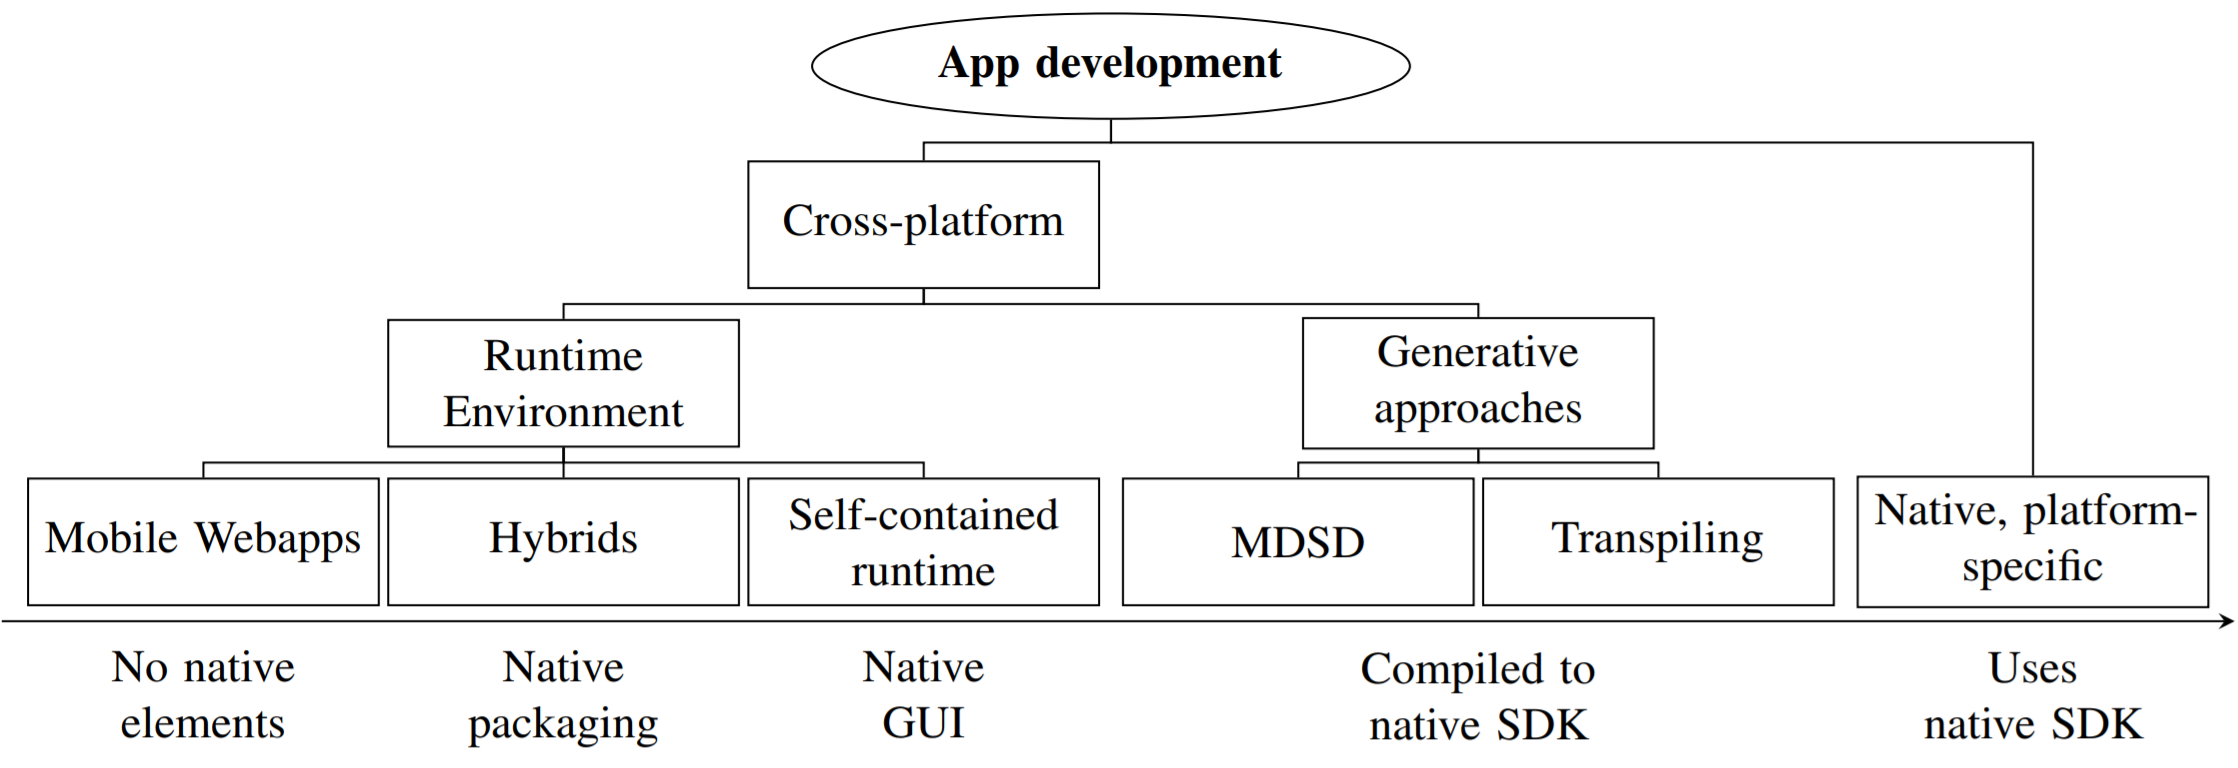
\includegraphics[scale=0.3]{kategorisierung_app_dev}
	\centering
	\caption[Kategorisierung von cross-plattform Entwicklungsansätzen]{Kategorisierung von cross-plattform Entwicklungsansätzen \cite{Majchrzak_category}}
	\label{fig:kategorisierung_app_dev}
\end{figure}

\newpage
\section{Native App-Entwicklung}

Die Native App-Entwicklung stellt zwar kein Framework dar, ist jedoch trotzdem wichtig zu erwähnen, da dies die ursprüngliche Art für ein mobiles Gerät zu entwickeln war und eine Referenz zu den folgenden Ansätzen darstellen soll.\\

Bei der nativen Entwicklung wird die Applikation mit den Technologien, Programmiersprachen und Tools entwickelt, welche von dem Hersteller der Zielplattform zur Verfügung gestellt wurden. Dafür wird ein \ac{SDK} genutzt, um die gewünschten Funktionen der Hardware zu benutzen und die passenden \ac{UI}-Elemente zu rendern und auf Eingaben des Nutzers zu reagieren. Jedoch ist der Quellcode an die jeweilige Zielplattform gebunden, da es sich um plattformspezifischen Bytecode handelt.
\begin{figure}[h]
	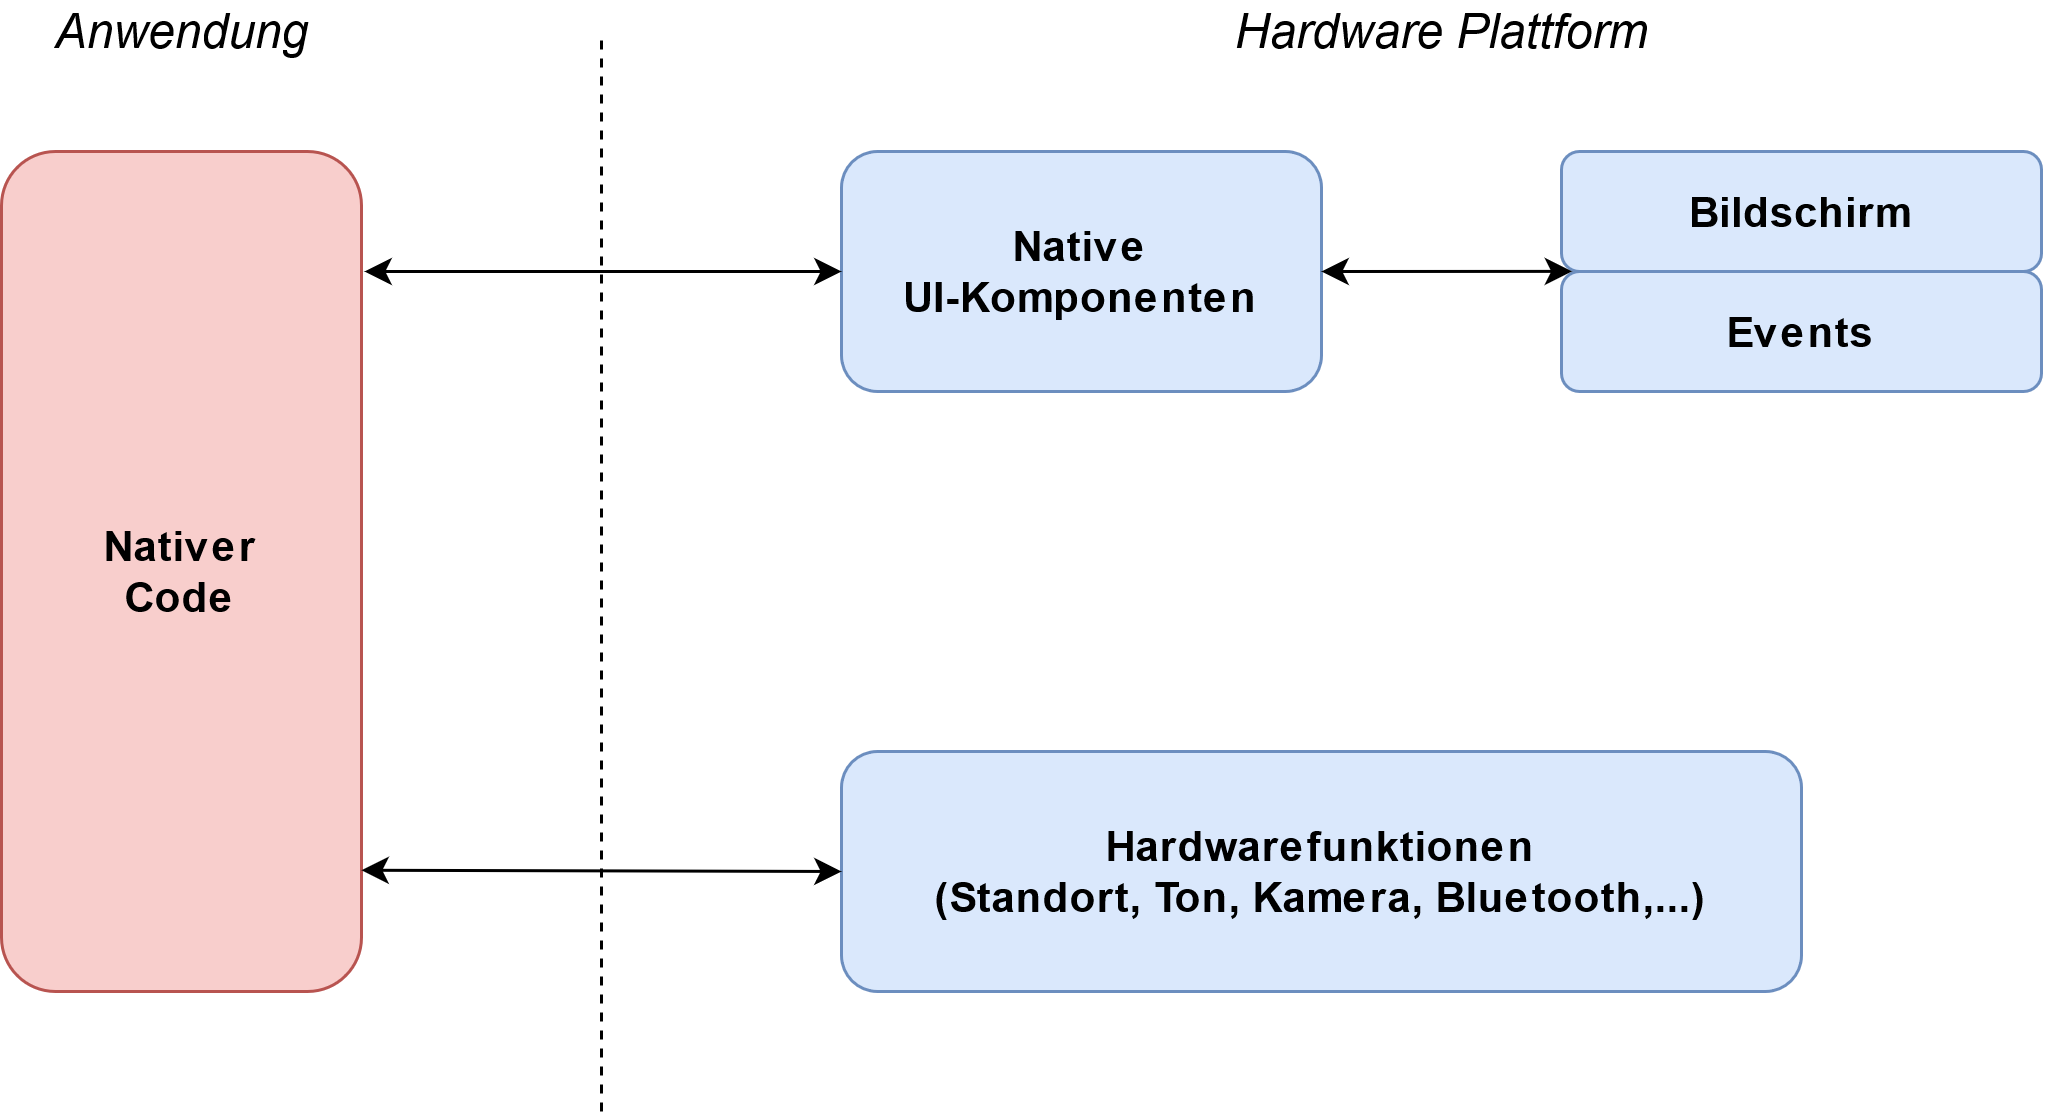
\includegraphics[scale=0.15]{native_framework}
	\centering
	\caption{Vereinfachtes Schema einer nativen Anwendung}
\end{figure}

Somit kann eine native Android Anwendung nur in Java oder Kotlin geschrieben werden, um zusammen mit dem Android \ac{SDK} die notwendige Funktionalität zu gewährleisten, während bei iOS Objective-C oder Swift benutzt werden muss, um zusammen mit Apples \ac{SDK} eine native Applikation zu erstellen\cite{rieger_evaluation}.\\

Die Native App wird anschließend im App-/Playstore des jeweiligen Betriebssystems veröffentlicht und kann von dort aus vom User heruntergeladen werden. Updates werden ebenfalls über diese Plattform verwaltet und dem User ausgespielt.

\makeatletter % Siehe https://tex.stackexchange.com/questions/19163/set-table-position-to-top
\setlength{\@fptop}{0pt}
\makeatother
\begin{table}[h]
	\begin{tabularx}{\linewidth}{>{\parskip1ex}X@{\kern4\tabcolsep}>{\parskip1ex}X}
		\toprule
		\hfil\bfseries Vorteile
		&
		\hfil\bfseries Nachteile
		\\\cmidrule(r{3\tabcolsep}){1-1}\cmidrule(l{-\tabcolsep}){2-2}
		
		%% PROS, seperated by empty line or \par
		Zugang zu allen Features der Zielplattform über die \ac{SDK} \ac{API}.\par
		Bestmögliche Performance auf dem Zielgerät, verglichen mit anderen Entwicklungsansätzen.\par
		Natives \glqq Look and Feel\grqq\  der \ac{UI}-Komponenten.\par
		Sofortiger Zugriff auf alle neuen Features der jeweiligen Zielplattform, sobald diese veröffentlicht werden.\par
		
		&
		
		%% CONS, seperated by empty line or \par
		Aufgrund der plattformspezifischen Tools muss dieselbe Applikation gleich zwei Mal entwickelt werden, was zu höherem Aufwand, längerer Entwicklungszeit, Notwendigkeit von zwei Entwicklungsteams mit Kenntnissen in verschiedenen Technologien und somit zu höheren Kosten führt.\par
		Native Apps sind komplexer in der Entwicklung und benötigen einen gewissen Grad an Erfahrung\cite{xanthopoulos_compare_cross_plattform}\par
		Einschränkungen und zusätzlichen Kosten, welche bei der Entwicklung und Veröffentlichung auf bestimmten Verteilungsplattformen entstehen. Da dies jedoch für jeden Ansatz gilt, welcher die App über den App-/Playstore verteilt wird dieser Aspekt im Folgenden nicht mehr explizit genannt.
		(Zugang zu Apples kostenpflichtigen Developer Program\cite{apple_member} und die Notwendigkeit eines Review-Prozesses von Apple, um eine App in dem App Store veröffentlichen zu können\cite{apple_submit})\par
		\\\bottomrule
	\end{tabularx}
	\caption{Vor- und Nachteile der nativen App-Entwicklung}
\end{table}

\clearpage
\section{Auf einer Laufzeitumgebung basierende Ansätze}
Bei dieser Oberkategorie an mobile App Frameworks wird eine Laufzeitumgebung genutzt, um eine übergeordnete Abstraktion der darunterliegenden Plattform zu schaffen. Somit können Anwendungen, welche darauf aufbauen eine einheitliche Schnittstelle verwenden und können somit Plattformübergreifend genutzt werden.
Diese Ansätze werden anhand der dafür genutzten Laufzeitumgebung weiter unterteilt.


\subsection{(Progressive) Web-App}

\subsubsection{\glqq Klassische\grqq\  Web-App}

Eine Web-App stellt eine Art einer Anwendung dar, welche innerhalb eines Browsers auf einem mobilen Gerät ausgeführt wird und mithilfe von Web-Technologie wie \ac{HTML}, \ac{CSS} und JavaScript erstellt wurde. Diese sind über einer \ac{URL} erreichbar und basieren, wie jede Website, auf dem klassischen Client-Server-Modell. Somit ist die Web-App komplett betriebssystemunabhängig, da lediglich ein aktueller Browser und eine Internetverbindung notwendig sind, um diese auf einem Endgerät zu nutzen. Dieser stellt somit die Laufzeitumgebung bereit, in der die Applikation ausgeführt wird. Dieser kümmert sich um die Darstellung und Verarbeitung von Inputs des Benutzers. Dabei werden keine nativen Features, welche über die Möglichkeiten des Browsers verwendet und es werden ebenfalls keine nativen \ac{UI}-Komponenten benutzt.\cite{waffa_tax_dev_approaches}.

\begin{figure}[h]
	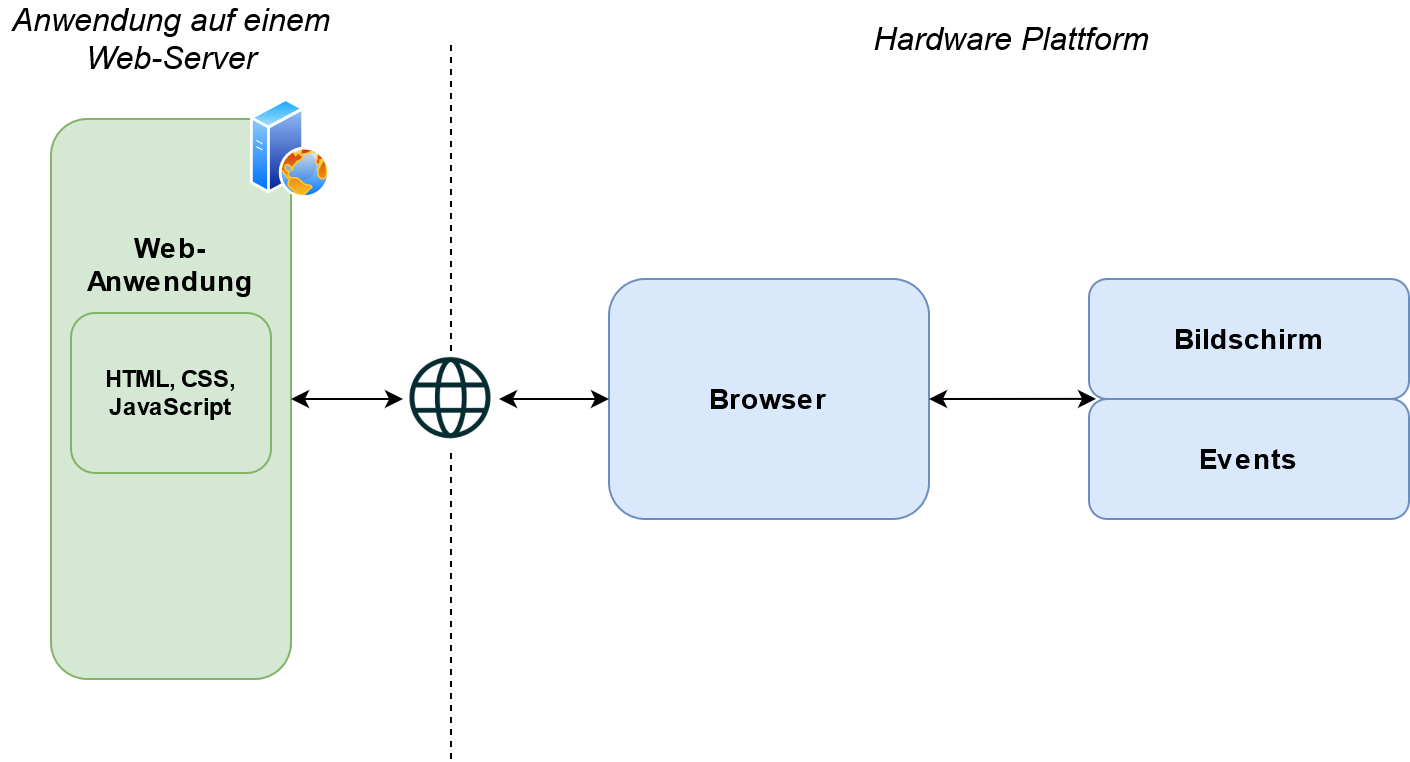
\includegraphics[scale=0.23]{web_app}
	\centering
	\caption{Vereinfachtes Schema einer Web-Anwendung}
\end{figure}

\begin{table}[h]
	\begin{tabularx}{\linewidth}{>{\parskip1ex}X@{\kern4\tabcolsep}>{\parskip1ex}X}
		\toprule
		\hfil\bfseries Vorteile
		&
		\hfil\bfseries Nachteile
		\\\cmidrule(r{3\tabcolsep}){1-1}\cmidrule(l{-\tabcolsep}){2-2}
		
		%% PROS, seperated by empty line or \par
		Die Verarbeitung geschieht auf einem Web-Server, sodass nur die \ac{UI}-Elemente an das Endgerät geschickt werden.\par
		Die Wartung der Anwendung ist leichter, da diese nur auf dem Web-Server liegt.\par
		Dieselbe Anwendung kann direkt in Browsern verschiedener Endgeräte angezeigt werden.\par
		
		&
		
		%% CONS, seperated by empty line or \par
		Sind nicht im App-/Playstore verfügbar.\par
		Eine Internetverbindung ist zwingend erforderlich.\par
		Schwächere Performance, da in einem Browser ausgeführt.\par
		Browserkompatibilität nicht überall gewährleistet.\par
		Keinen Zugriff auf alle Hardwarefunktionen, sondern sind auf die des Browsers beschränkt.\par
		\\\bottomrule
	\end{tabularx}
	\caption{Vor- und Nachteile einer \glqq klassischen\grqq\ Web-App}
\end{table}

\newpage
\subsubsection{Progressive Web-App}

Der Name Progressive Web-App ist kein allgemein definierter Begriff. Dieser wurde 2015  von dem Google Entwickler Alex Russell eingeführt, um eine sich an das Endgerät anpassende Web-Applikation zu beschreiben, welche ausschließlich aus Web-Technologien wie unter anderem JavaScript, \ac{CSS} und \ac{HTML} besteht. Zusätzlich erweitert die \ac{PWA} den Funktionsumfang einer Web-App um Verhaltensweisen und Features, welche Traditionell den nativen Apps vorbehalten waren. Dazu gehören u.A. das Hinzufügen zu dem Homescreen, eine Möglichkeit die Website auch ohne Internet zu bedienen, und Push-Benachrichtigungen zu erhalten\cite{mozilla_pwa}. Besonders hervorzuheben ist die Tatsache, dass der User selbst entscheidet, ob diese Features genutzt werden sollen oder nicht. 

\blockcquote{firtman_mobile_web}{
	A PWA is a Website running in a browser that will progressively add more features based on compatibility.
}


Dabei stellt die Progressive Web-App keine einzige Technologie dar, sondern eher eine Ansammlung an Eigenschaften, welche erfüllt werden sollten, um als eine \ac{PWA} bezeichnet werden zu können. Die Kriterien welche Google für eine \ac{PWA} nennt sind in zwei Kategorien aufgeteilt. Kernanforderungen an die Website und Zusatzanforderungen welche eine \glqq optimale\grqq\ \ac{PWA} ausmachen.\\


\begin{table}[!h]
	\begin{tabularx}{\linewidth}{>{\parskip1ex}X@{\kern4\tabcolsep}>{\parskip1ex}X}
		\toprule
		\hfil\bfseries Kernanforderungen
		&
		\hfil\bfseries Zusätzliche Anforderungen
		\\\cmidrule(r{3\tabcolsep}){1-1}\cmidrule(l{-\tabcolsep}){2-2}
		
		%% Kernanforderungen, seperated by empty line or \par
		Geschwindigkeit\par
		Erreichbarkeit von jedem Browser und Endgerät\par
		Responsive Anpassung an die Bildschirmgröße\par
		Offline-Funktionalität\par
		Installierbarkeit\par
		
		&
		
		%% zusätzliche Anforderungen, seperated by empty line or \par
		Barrierefreiheit\par
		Sicherheit\par
		Sichtbarkeit (z.B. über Googles Suchfunktion)\par
		Transparenz bezüglich der erforderlichen Berechtigungen\par
		\\\bottomrule
	\end{tabularx}
	\caption[Anforderungen an eine \ac{PWA}]{Anforderungen an eine \ac{PWA}\cite{google_pwa_check}}
\end{table}

\newpage
Zu den technischen Bestandteilen, welche eine \ac{PWA} von einer Web-App unterscheiden gehören:\\

\begin{enumerate}
	\item Die App Shell - Stellt das minimale \ac{HTML}, \ac{CSS} und JavaScript Gerüst dar, in welchem der Content der \ac{PWA} angezeigt werden soll. Sie ist dafür zuständig die statischen Inhalte der Anwendung anzuzeigen, welche im Nutzungsverlauf der \ac{PWA} gleich bleiben. Dazu gehört üblicherweise die Navigationsleiste oder die Homepage. Diese werden lokal auf dem Endgerät abgelegt, sodass Ladezeiten minimiert werden können.
	
	\item Der Service Worker - Ein Hintergrunddienst in JavaScript geschrieben, welcher auch bei geschlossener App weiterläuft. Dieser wird beim Abruf der \ac{PWA} mitgeliefert und genutzt, falls die \ac{PWA} \glqq zum Homescreen hinzugefügt\grqq\ wird. Er hat die Aufgabe Netzwerkanfragen abzufangen und passend zu verarbeiten. Außerdem verwaltet der Service Worker den Cache, wodurch Anfragen auch ohne Internet verarbeitet und beantwortet werden können, um die offline Funktionalität zu ermöglichen. Laut Biørn-Hansen et. al., 2017\cite{hansen_pwa} kann eine \ac{PWA} ohne Service Worker nicht richtig funktionieren. Damit ist der Service Worker der zentrale Bestandteil einer \ac{PWA}. 
	
	\item Das Web Application Manifest - 
	Eine Datei, welche es dem Entwickler ermöglicht das Verhalten und Aussehen der \glqq installierten\grqq\ \ac{PWA} auf dem mobilen Gerät des Users anzupassen. Dazu gehören u.A. das angezeigte Logo auf dem HomeScreen oder verschiedenen Caching-Strategien.
	
\end{enumerate}

\begin{figure}[!ht]
	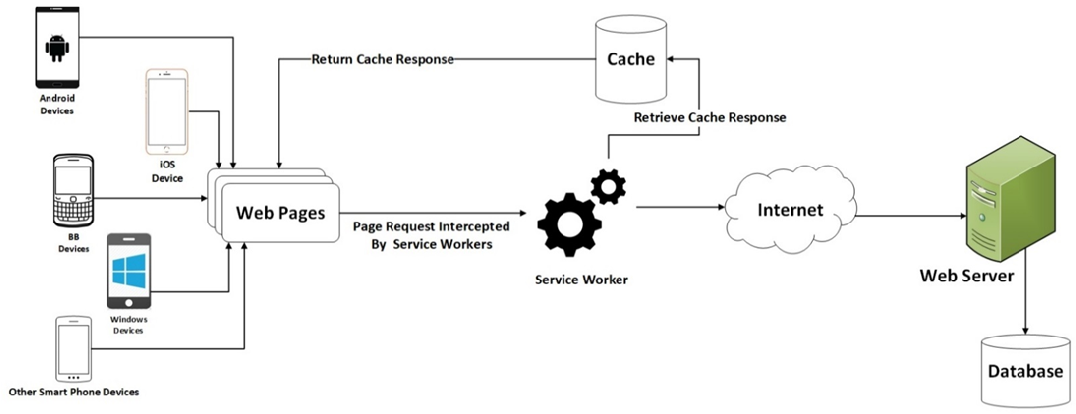
\includegraphics[scale=0.45]{pwa_aufbau}
	\centering
	\caption[Technischer Aufbau einer \ac{PWA}]{Technischer Aufbau einer \ac{PWA} \cite{adetunji_pwa}}
\end{figure}


\begin{table}[ht!]
	\begin{tabularx}{\linewidth}{>{\parskip1ex}X@{\kern4\tabcolsep}>{\parskip1ex}X}
		\toprule
		\hfil\bfseries Vorteile
		&
		\hfil\bfseries Nachteile
		\\\cmidrule(r{3\tabcolsep}){1-1}\cmidrule(l{-\tabcolsep}){2-2}
		
		%% PROS, seperated by empty line or \par
		Eine \ac{PWA} lässt sich auch ohne Internetverbindung benutzen.\par
		Die \ac{PWA} ist leicht erreichbar und teilbar, da diese über einen Link im Browser abgerufen werden kann.\par
		Es ist möglich bereits bestehende Webseite zu einer \ac{PWA} umzuwandeln.\par
		Funktionen wie \glqq zum Homescreen hinzugefügen\grqq\ oder Push-Benachrichtigungen führen dazu, dass der Nutzer die Web-App als native Anwendung wahrnimmt und anders mit dieser interagiert\cite{medium_pwa_pro_con}.\par
		Eine \ac{PWA} benötigt zwingend \ac{HTTPS}, was die Datenübertragung vor \glqq man-in-the-middle\grqq\ Attacken zusätzlich schützt.\par
		
		&
		
		%% CONS, seperated by empty line or \par
		\ac{PWA}s haben keinen Zugriff auf alle Hardwarefunktionen, sondern sind auf die des Browsers beschränkt.\par
		Sind nicht im App-/Playstore verfügbar.\par
		Schwächere Performance, da in einem Browser ausgeführt.\par
		\ac{PWA}s sind derzeit noch nicht auf allen Geräten und Browsern komplett unterstützt.\par
		\\\bottomrule
	\end{tabularx}
	\caption[Vor- und Nachteile einer \ac{PWA}]{Vor- und Nachteile einer \ac{PWA}\cite{adetunji_pwa}}
\end{table}

\clearpage
\subsection{Hybride App}

Hybride Apps stellen eine Kombination von Web-Apps und nativen Apps dar. Diese verwenden, ebenfalls vorwiegend Web-Technologien. Der Quelltext  wird ebenfalls innerhalb eines Browsers ausgeführt. Jedoch handelt es sich dabei nicht um den bereits installierten Browser wie bei Web-Apps, sondern um einen plattformspezifischen Container (UIWebView unter iOS und WebView unter Android)\cite{xanthopoulos_compare_cross_plattform}. Dieser wird bei dem Download der App aus dem App-/Playstore zusammen mit dem Quellcode der App im Hintergrund bereitgestellt und stellt die Laufzeitumgebung dar. Die \ac{UI}-Komponenten werden weiterhin von dem Container gerendert, obwohl manche Frameworks versuchen diese möglichst nativ aussehen zu lassen. Um die Limitierungen des Zugriffes auf bestimmte Hardware oder Informationen aus dem Browser heraus zu umgehen, wird mithilfe eines \grqq Überbrückungs-Moduls\grqq\ auf den nativen Teil der Anwendung zugegriffen. Dieser hat Zugriff auf die nativen APIs der Plattform. Dies führt, je nachdem wie aktive diese verwendet wird, zu einem Performance-Engpass, welcher in \foreignlanguage{ngerman}{\cref{react}} näher erläutert wird. Jedoch ist dieser Teil der Hybriden App wiederum plattformspezifisch. Allerdings stellen cross-plattform Frameworks diese Funktionalität direkt bereit und nehmen dem Entwickler viel Arbeit ab, sodass es bei der Entwicklung selten notwendig ist nativen Code selbst zu schreiben\cite{kmu_fh_joanneum}.

\begin{figure}[!h]
	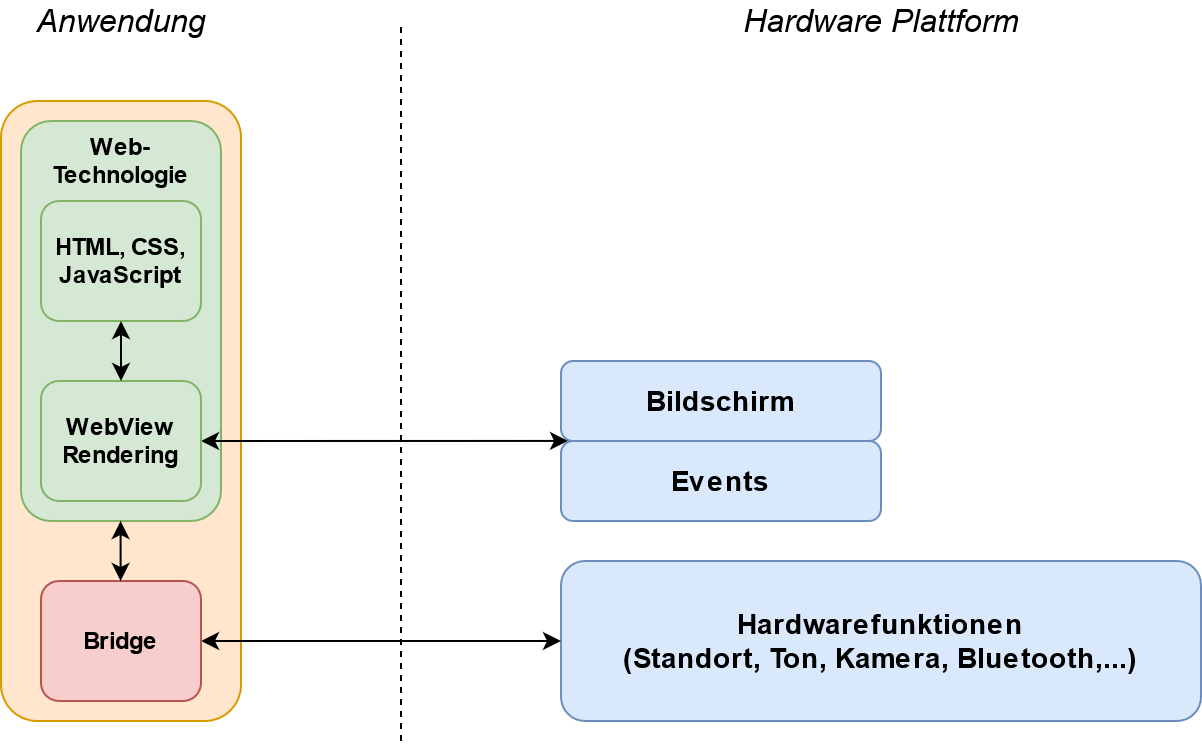
\includegraphics[scale=0.25]{hybrid_app}
	\centering
	\caption{Vereinfachtes Schema einer hybriden App}
\end{figure}

\begin{table}[!h]
	\begin{tabularx}{\linewidth}{>{\parskip1ex}X@{\kern4\tabcolsep}>{\parskip1ex}X}
		\toprule
		\hfil\bfseries Vorteile
		&
		\hfil\bfseries Nachteile
		\\\cmidrule(r{3\tabcolsep}){1-1}\cmidrule(l{-\tabcolsep}){2-2}
		
		%% PROS, seperated by empty line or \par
		Kann über den App-Store verteilt werden, sowie als Web-App bereitgestellt werden.\par
		Für die Implementierung und Tests kann größtenteils der Desktop-Browser genutzt werden.\par
		Hat Zugriff auf vom Framework unterstützten Hardwarefunktionen.\par
		Die Anwendung hat auf verschiedenen Endgeräten ein einheitliches \ac{UI}/\ac{UX}, da der Inhalt mit Web-Technologie definiert und in einem browserähnlichem Container dargestellt wird.\par
		Eine bereits bestehende Webseite kann in kurzer Zeit zu einer hybriden App umgewandelt werden.\par
		
		&
		
		%% CONS, seperated by empty line or \par
		Schwächere Performance, da die App innerhalb einer Browser-Engine ausgeführt wird und manipulationen des \ac{DOM}s viel Zeit kosten.\par
		Häufige Nutzung nativer Funktionen kann ebenfalls die Performance beeinflussen.\par
		Mehr Fehlerquellen durch Nutzung verschiedener Technologien, welche sich je nach Plattform unterschiedlich verhalten kann.\par
		Kein Zugriff auf native \ac{UI}-Elemente.\par
		\\\bottomrule
	\end{tabularx}
	\caption{Vor- und Nachteile einer hybriden App}
\end{table}

\clearpage %Macht komische freistellen siehe https://tex.stackexchange.com/questions/2958/why-is-newpage-ignored-sometimes
\subsection{Eigenständige Laufzeitumgebung}

Im Gegensatz zu der (progressiven) Web-App und dem hybriden Ansatz greift diese Art der Anwendung nicht mehr auf die üblichen Web-Technologien zurück und rendert den Inhalt nicht innerhalb eines Browsers oder browserähnlichen Containers, sondern stellt eine vollständig eigenständige Laufzeitumgebung zur Verfügung. Somit wird es den Entwicklern der Applikation ermöglicht Programmiersprachen wie JavaScript (z.B. React Native) oder C\# (z.B. Xamarin) zu verwenden. Um das Übersetzen der Aufrufe aus dem plattformunabhängigen Quellcode in das passende native Äquivalent kümmert sich ein \grqq Überbrückungs-Modul\grqq\ oder \ac{API} des Frameworks. Dies führt jedoch, je nach Verwendungshäufigkeit, ebenfalls zu einem Performance-Engpass, welcher in \foreignlanguage{ngerman}{\cref{react}} näher erläutert wird. Die Laufzeitumgebung deckt somit einen größeren Aufgabenbereich als der hybride Ansatz ab und ist somit flexibler, da hierbei das Rendern der \ac{UI} mit nativen Elementen realisiert werden kann.\cite{hansen_performance_overhead_cross_platform}


\begin{figure}[!h]
	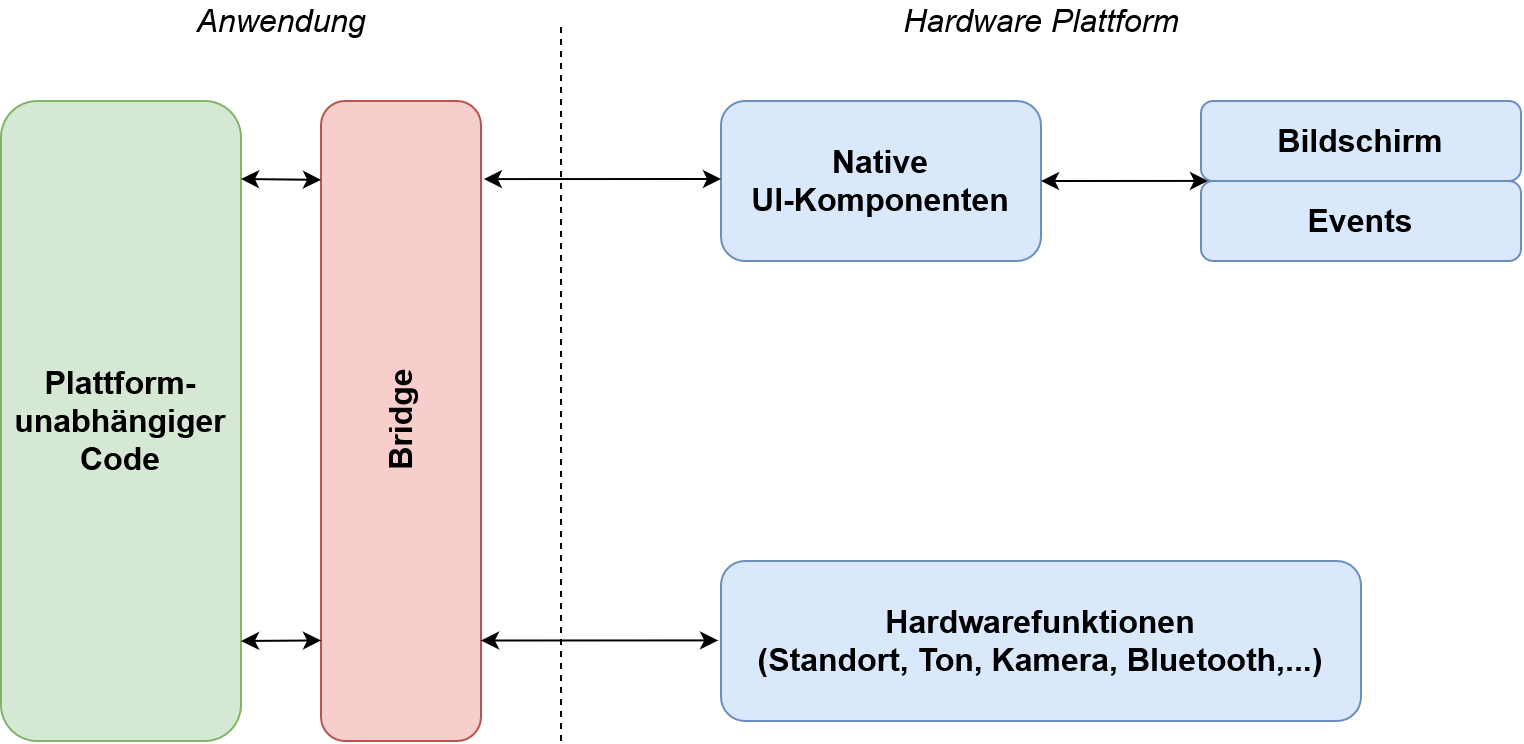
\includegraphics[scale=0.21]{eigenstaendige_laufzeitumgebung}
	\centering
	\caption{Vereinfachtes Schema einer App mit eigener Laufzeitumgebung}
\end{figure}


\begin{table}[h]
	\begin{tabularx}{\linewidth}{>{\parskip1ex}X@{\kern4\tabcolsep}>{\parskip1ex}X}
		\toprule
		\hfil\bfseries Vorteile
		&
		\hfil\bfseries Nachteile
		\\\cmidrule(r{3\tabcolsep}){1-1}\cmidrule(l{-\tabcolsep}){2-2}
		
		%% PROS, seperated by empty line or \par
		Es besteht kein Zwang Web-Technologien verwenden zu müssen.\par
		Die Anwendung kann über den App-/Playstore verteilt werden.\par
		Es können native \ac{UI}-Elemente verwendet werden.\par
		Es sind vom Framework unterstützten Hardwarefunktionen verfügbar.\par
		
		&
		
		%% CONS, seperated by empty line or \par
		Komplexe Frameworks, da diese mehrere verschiedene Aufgaben übernehmen.\par
		Je nach Kenntnisstand höherer Einarbeitungsaufwand.\par
		Performance leidet unter der Notwendigkeit mit nativen Komponenten über die Bridge kommunizieren zu müssen.\par
		Initiale Startzeit der App ist hoch, da aufgrund der erhöhten Komplexität eine größere Codebasis interpretiert und \ac{JIT} kompiliert werden muss.\par
		\\\bottomrule
	\end{tabularx}
	\caption{Vor- und Nachteile einer App mit eigenständiger Laufzeitumgebung}
\end{table}

\newpage
\section{Generierende Ansätze}

Bei diesen Ansätzen wird es dem Entwickler ermöglicht eine Applikation einmalig zu entwickeln und daraus nativen Code für die jeweilige Zielplattform zu generieren.
Dabei wird zwischen modellgetriebenen und cross-kompilierenden Ansätzen weiter unterschieden.

\subsection{Modellgetrieben}

Bei diesem Ansatz wird die Applikation in einer Modellierungssprache (Textuell oder Grafisch) plattformunabhängig definiert.
Hierbei kann wiederum in zwei Gruppen unterteilt werden: Mehrstufig und einstufig generierende Ansätze. \\

Bei der Einstufigen Code Generation wird aus der Modellierungssprache mit Hilfe von mehreren Codegeneratoren nativer Quellcode für die jeweilige Zielplattform erzeugt. Beispiele dafür wären MD2, MobML oder Mobl.\\

Bei der Mehrstufigen Code Generation wird Quellcode für ein weiteres Cross-Plattform Framework erzeugt. Daraus wird in einem weiteren Schritt wiederum Quellcode für die jeweilige Zielplattform erzeugt. Ein Beispiel für solch ein Framework wäre AXIOM.\\

Diese Ansätze sind jedoch als Spezialfälle zu betrachten und werden vorwiegend akademisch Diskutiert. Kommerzielle Ansätze existieren haben jedoch alle eigene Modellierungssprachen, wodurch sich diese Ansätze nicht durchsetzen konnten\cite{umuhoza_modell}\cite{hansen_performance_overhead_cross_platform}.\\

\begin{table}[h]
	\begin{tabularx}{\linewidth}{>{\parskip1ex}X@{\kern4\tabcolsep}>{\parskip1ex}X}
		\toprule
		\hfil\bfseries Vorteile
		&
		\hfil\bfseries Nachteile
		\\\cmidrule(r{3\tabcolsep}){1-1}\cmidrule(l{-\tabcolsep}){2-2}
		
		%% PROS, seperated by empty line or \par
		Definition der Applikation auf einem sehr hohen und abstrakten Level möglich.\par
		Keine Notwendigkeit Code zu schreiben.\par
		Sehr hohe Entwicklungsgeschwindigkeit bei Entwicklung von Prototypen möglich.\par

		&
		
		%% CONS, seperated by empty line or \par
		Zersplitterte Framework-Landschaft.\par
		Fehleranfällig, da viele verschiedene Technologien aufeinander aufbauen.\par
		Können häufig nur die Features anbieten, welche auf allen Plattformen verfügbar sind.\par
		Kleine Community und wenig Hilfsmaterialien, daher vorwiegend akademisch Diskutiert.\par
		
		\\\bottomrule
	\end{tabularx}
	\caption{Vor- und Nachteile einer modellgetriebenen App}
\end{table}


\newpage
\subsection{Cross-Kompilierend}

Bei diesem Ansatz wird versucht den geschrieben Quellcode der Anwendung in eine, für die Zielplattform passende Repräsentation umzuwandeln. Dies kann auf verschiedenen Abstraktionsebenen des Quellcodes geschehen. Daher wird in der Literatur der Begriff kompilierend oder transpilierend benutzt. Bei der Kompilation wird meist Quellcode einer niedrigeren Abstraktionsstufe erzeugt wird, während bei der Transpilation Quellcode häufig auf ähnlicher Abstraktionsstufe erzeugt wird. Diese Trennung ist jedoch nicht einheitlich definiert und ist daher häufig kontextabhängig. Allerdings fokussieren sich solche Ansätze die Regel nur auf einen bestimmten Aspekt der Anwendung, sodass noch zusätzliche Schritte notwendig sind, um eine vollständige App zu erzeugen. Ein Beispiel dafür ist Googles J2ObjC \cite{hansen_performance_overhead_cross_platform}.
Besonders hervorzuheben ist dabei Googles Flutter Framework, bei welchem die Applikation in Dart geschrieben wird. Dieses ist der jüngste Vertreter dieser Kategorie. Eine Besonderheit bei Flutter besteht darin, dass keine Nativen Komponenten gerendert werden. Das Framework überlässt diese Aufgabe komplett der mitgelieferten Skia Graphics Engine. Daraus folgt eine erhöhte Flexibilität und Performance\cite{medium_rendering_flutter}. \\

\begin{table}[h]
	\begin{tabularx}{\linewidth}{>{\parskip1ex}X@{\kern4\tabcolsep}>{\parskip1ex}X}
		\toprule
		\hfil\bfseries Vorteile
		&
		\hfil\bfseries Nachteile
		\\\cmidrule(r{3\tabcolsep}){1-1}\cmidrule(l{-\tabcolsep}){2-2}
		
		%% PROS, seperated by empty line or \par
		Ähnliche Performance zu nativen Apps möglich.\par
		Es können native \ac{UI}-Elemente verwendet werden.\par
		
		&
		
		%% CONS, seperated by empty line or \par
		Es werden, je nach Framework, nur eine Begrenze Anzahl an Plattformen unterstützt.\par
		Es werden nur Features unterstützt, welche auf allen Plattformen verfügbar sind.\par
		Legen den Fokus teilweise nur auf einen bestimmten Aspekt der Anwendung, sodass noch weitere Schritte notwendig sind, um eine vollwertige App zu erzeugen.\par
		\\\bottomrule
	\end{tabularx}
	\caption{Vor- und Nachteile einer cross-kompilierenden App}
\end{table}